\documentclass[11pt]{article}

\usepackage{geometry, fancyhdr, tikz, float}
\usetikzlibrary{snakes}

\title{The Ekans Webserver \\ {\small\textbf{Software Design Specification}}}
\author {Samuel C. Payson}
\date{{\footnotesize \emph{last modified\\}}\today}

\begin{document}
\maketitle
\thispagestyle{empty}
\pagebreak
\pagestyle{fancy}
\setcounter{page}{1}
\pagenumbering{roman}
\tableofcontents
\pagebreak
\setcounter{page}{1}
\pagenumbering{arabic}
\section{Introduction}
Ekans is a lightweight webserver designed to quickly serve static content, while allowing for dynamic content powered by a Python backend. The initial section of this document provides a concise high-level overview of the server's design, followed by more detailed sections explaining the implementation of each of the server's main modules.
\subsection{The Ekans Design Mentality}
As a large project written in C, Ekans adhere's primarily to the mindset of the procedural paradigm. This means that data and procedures are seperate components of each module. In our model, modules exist as a set of procedures which communicate with eachother through changes that they make to data.

The main function of Ekans is the processing and communication of hypertext data. Because of this focus, our design places emphasis on the movement of data around the system. Modules are seperated based on the order and nature of their interactions with data.

\subsection{Understanding Figures}
The flow-charts and figures throughout this document attempt to follow the same general guidelines for design in order to be as useful as possible. The following are a set of informal rules for the interpretation of figures. \emph{Do not take this to be the absolute truth!} 

\pagebreak

\section{Overview}

\subsection{The Main Modules}
The two main modules of Ekans are known as \emph{dispatch} and the \emph{agent pool}. Dispatch is responsible for establishing connections with new clients and handing them off to agents. The agents handle individual clients one at a time, serving their requests and dealing with errors.

\begin{figure}[H]
  \begin{center}
    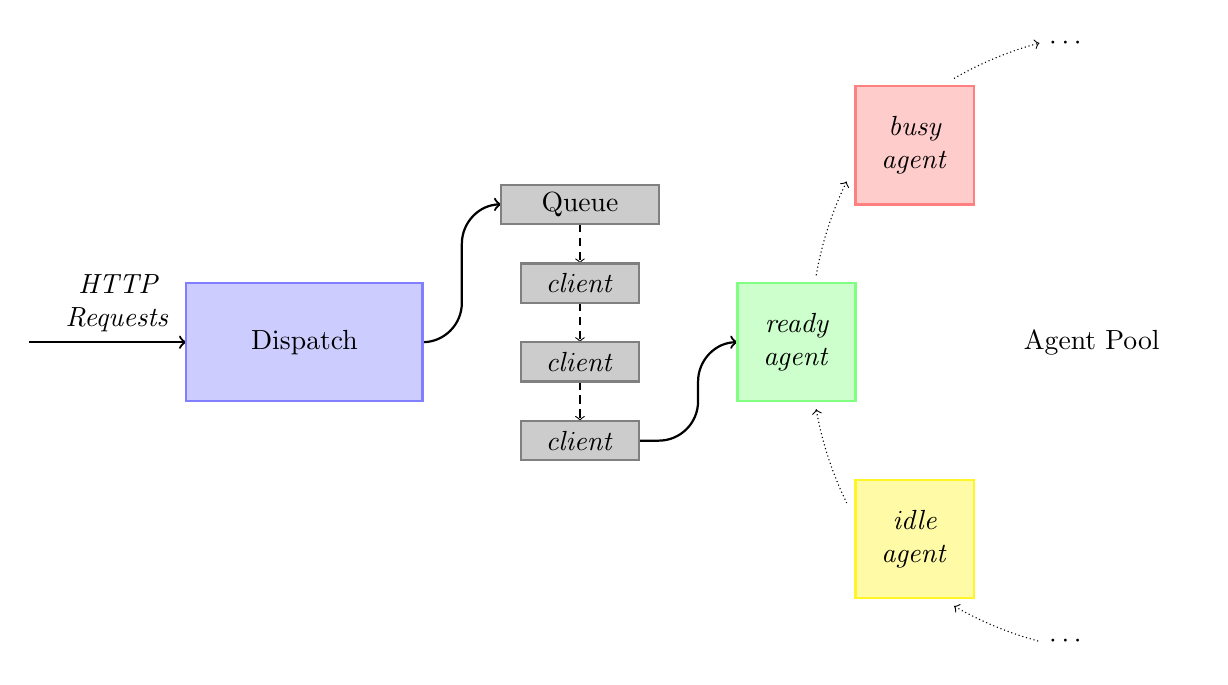
\begin{tikzpicture}[
        thick,
        queue/.style={fill=black!20,draw=black!50},
      ]


      \draw[->,thick] (-5, 0) node[above right, text width=2cm, text centered] {\emph{HTTP Requests}} -- (-3, 0);
      \draw[densely dashed,->,thin] (2, 1.5) -- (2, 1);
      \draw[densely dashed,->,thin] (2, 0.5) -- (2, 0);
      \draw[densely dashed,->,thin] (2, -0.5) -- (2, -1);
      \draw[->,thick] (0, 0) arc (-90:0:0.5cm) -- (0.5,1.25) arc (180:90:5mm);
      \draw[->,thick] (2.75,-1.25) -- ++(0.25,0) arc (-90:0:5mm) -- ++(0, 0.25) arc (180:90:5mm);
      \draw[densely dotted,thin,->] (5, 0.85) arc (170:154:45mm);
      \draw[densely dotted,thin,->] (6.75, 3.35) arc (120:105:45mm) node[right] {$\cdots$};
      \draw[densely dotted,thin,<-] (5, -0.85) arc (190:206:45mm);
      \draw[densely dotted,thin,<-] (6.75, -3.35) arc (240:255:45mm) node[right] {$\cdots$};

      \draw[draw=blue!50,fill=blue!20] (-3,-0.75) rectangle (0,0.75);
      \draw[queue] (1, 2) rectangle (3, 1.5);
      \draw[queue] (1.25, 1) rectangle (2.75, 0.5);
      \draw[queue] (1.25, 0) rectangle (2.75, -0.5);
      \draw[queue] (1.25, -1) rectangle (2.75, -1.5);
      \draw[draw=red!50,fill=red!20] (5.5, 1.75) rectangle (7, 3.25);
      \draw[draw=green!50,fill=green!20] (4, 0.75) rectangle (5.5, -0.75);
      \draw[draw=yellow!85,fill=yellow!35] (5.5, -1.75) rectangle (7, -3.25);

      \path (-1.5, 0) node {Dispatch};

      \path (2, 1.75) node {Queue};
      \path (2, 0.75) node {\emph{client}};
      \path (2,-0.25) node {\emph{client}};
      \path (2,-1.25) node {\emph{client}};
      \path (6.25, 2.5) node[text centered,text width=1.5cm] {\emph{busy agent}};
      \path (6.25, -2.5) node[text centered,text width=1.5cm] {\emph{idle agent}};
      \path (4.75, 0) node[text centered,text width=1.5cm] {\emph{ready agent}};
      \path (8.5, 0) node[text centered,text width=2.5cm] {Agent Pool};

    \end{tikzpicture}
  \end{center}\caption{High level interactions of dispatch and the agent pool.}\label{fig:agent-dispatch-flow}
\end{figure}

\end{document}
